\chapter{Обзор современных результатов в области сравнительной геномики и геномных перестроек}

\section{Виды геномных перестроек}

Геномные перестройки (англ. \textit{genome rearrangements}) ~--- это эволюционные события, которые меняют порядок генов на хромосомах.
Некоторые хромосомные области более подвержены перестройкам, чем другие.
Эта неустойчивость, как правило, обусловленая склонностью этих областей к смещению во время восстановления ДНК, усугубляется дефектами появления реплицирующих белков, которые повсеместно влияют на целостность генома.

\begin{figure}[h!]
    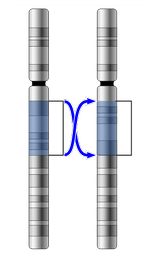
\includegraphics[width=1.5in]{img/reversal.png}
    \caption{Реверсия}
    \label{reversal}
\end{figure}

Самые распространенные геномными перестройками являются:
\begin{enumerate}
    \item Реверсия (инверсия) (англ. \textit{reversal}) ~--- разворот сегмента (рис.~\ref{reversal});
    \item Транслокация ~--- (анлг. \textit{translocation}) попарная замена сегментов двух хромосом;
    \item Слияние (англ. \textit{fusion}) ~--- объединение двух хромосом в одну;
    \item Расщепление (англ. \textit{fission}) ~--- разделение одной хромосомы на две.
\end{enumerate}

Все эти четыре типа перестановок могут быть смоделированы операцией Двойное-Разрезание-и-Склеивание (ДРС) (англ. \textit{Double-Cut-and-Join}) \cite{dcj}, которая <<разрезает>> хромосому в двух локациях и склеивает полученные регионы в другом порядке.

Также существуют более сложные геномные перестройки, которые могут быть смоделированы как разрез хромосом в $k$ локациях, где $k>2$, и склеивание полученных регионов в другом порядке.
Например, транспозиция (англ. \textit{transposition}).
В рамках данной работы эти перестройки рассматриваться не будут ввиду того, что происходят они достаточно редко, но при этом сильно усложняют получившуюся модель.
Рассмотрены будут все виды геномных перестроек, моделируемые с помощью ДРС, то есть $k=2$.

\section{Существующие методы оценки эволюционного расстояния}

\begin{figure}[h!]
    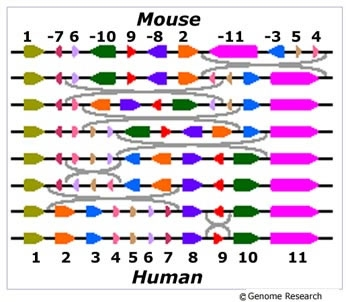
\includegraphics[width=4in]{img/mouse_human.jpg}
    \caption{Эволюционный сценарий}
    \label{mouse-human}
\end{figure}

Для любой оценки расстояния между двумя геномами мы предполагаем, что они имеют в себе одинаковый набор блоков, организованных в разном порядке.
Задача оценки расстояния сводится к задаче об оценке необходимого количества операций ДРС на соответствующих данным геномам графах.

\subsection{Оценка через минимальное расстояние}
Первым был предложен подход оценки расстояния как минимального необходимого, то есть минимального количества необходимых операций ДРС для перестройки одного генома в другой.
Появление данного подхода весьма закономерно и на данный момент используется в качестве нижней границы для оценки результатов.
Для геномов, которые слабо удалены друг от друга, данный метод даёт хорошие результаты.

Минимальное растоние определяется через <<граф точек разрыва>> (англ. \textit{breakpoint graph}.
Для восстановления эволюционного сценария решается задача сортировки.
Подобная задача сортировки с ипользованием только инверсий является NP-полной \cite{sorting-is-difficult}.

Но если рассматривать геномы, которые достаточно далеко удалены друг от друга, то ошибка даного алгоритма становится заметно выше.
Когда в реальности между генами могло произойти весьма большее количество перестроек, а природа их происхождения является случайной и не ведёт самым коротким путём, алгоритм оценки через минимальное расстояние будет же искать минимальный путь, который может отличаться от реального.

При большом количестве шагов ошибка данного метода в рамках модели, предложенной в данной работе, может достигать $50 \, \%$.
Но необходимо отметить, что с увеличением числа шагов происходит <<насыщение>> (англ. \textit{saturation}) модели, и любой алгоритм оценки расстояния начинает давать более плохие результаты.
В рамках построенной модели мы будем сравнивать получившийся алгоритм оценки с методом оценки через минимальное расстояние.

\subsection{Модель поломки случайных регионов}

В статье \cite{termin} был предложен метод для оценки истинного эволюционного расстояния, а также преложен сам термин <<истинного эволюционного расстояния>> (англ. \textit{true evolutionary distance}).
Однако, данный метод полагает, что геномы могут быть поломаны в любой позиции с равной вероятностью, то есть весь геном является <<хрупким>>.
Данное предположение, известное как модель поломок случайных регионов (ПСР-модель) (англ. \textit{random breakage model}) эволюции хромосом, было опровергнуто в пользу более строгой модели поломок хрупких регионов (ПХР-модели) (англ. \textit{fragile breakage model}) \cite{mouse}, в которой утверждается, что только определенные <<хрупкие>> (англ. \textit{fragile}) геномные области подвержены к перестановкам.
ПХР-модель поддерживается многими недавними исследованиями различных геномов (например, \cite{fragile}).
ПСР-модель можно рассматривать как экстремальный случай ПХР-модели, где каждая геномная область является хрупкой.

Таким образом, хотя в данной статье и был предложен алгоритм оценки, он не учитывает того факта, что некоторые регионы генома могут быть <<прочными>> (англ. \textit{solid}) и не имеют возможности сломаться. С точки зрения биологии это означает, что подобные изменения критичны и, скорее всего, ведут к гибели организма.

\subsection{Модель поломки хрупких регионов}
В статье \cite{alexeev-1} предложен новый метод оценки истинного эволюционного расстояния между двумя геномами в рамках ПХР-модели (модель поломки хрупких регионов).
Произведено оценивание предложенного метода для имитируемых геномов, которые показывают его высокую точность.

Для оценки истинного эволюционного расстояния в данной модели используется анализ так называемого <<графа точек разрыва>>.
Аналитически выведены формулы для распределения необходимых для оценки компонент и на основании этих формул преложен аналитический метод оценки истинного эволюционного расстояния.

Так как изучаемая нами модель является развитием и уточнением ПХР-модели, далее ПХР-модель будет рассмотрена подробнее.

\section{Анализ модели поломки хрупких регионов}
\subsection{Граф точек разрыва и двойной-разрез-и-склеивание}
Анализ начинается с круговых геномов и позже обращается к линейным геномам.
Геном с $n$ блоками представляется в виде графа генома, состоящего из $n$ направленных блоковых рёбер (англ. \textit{block edges}), кодирующих блоки и их границы, и $n$ неориентированных рёбер смежности (англ. \textit{adjacency edges}), кодирующих смежности между блоками.

\begin{figure}[h!]
    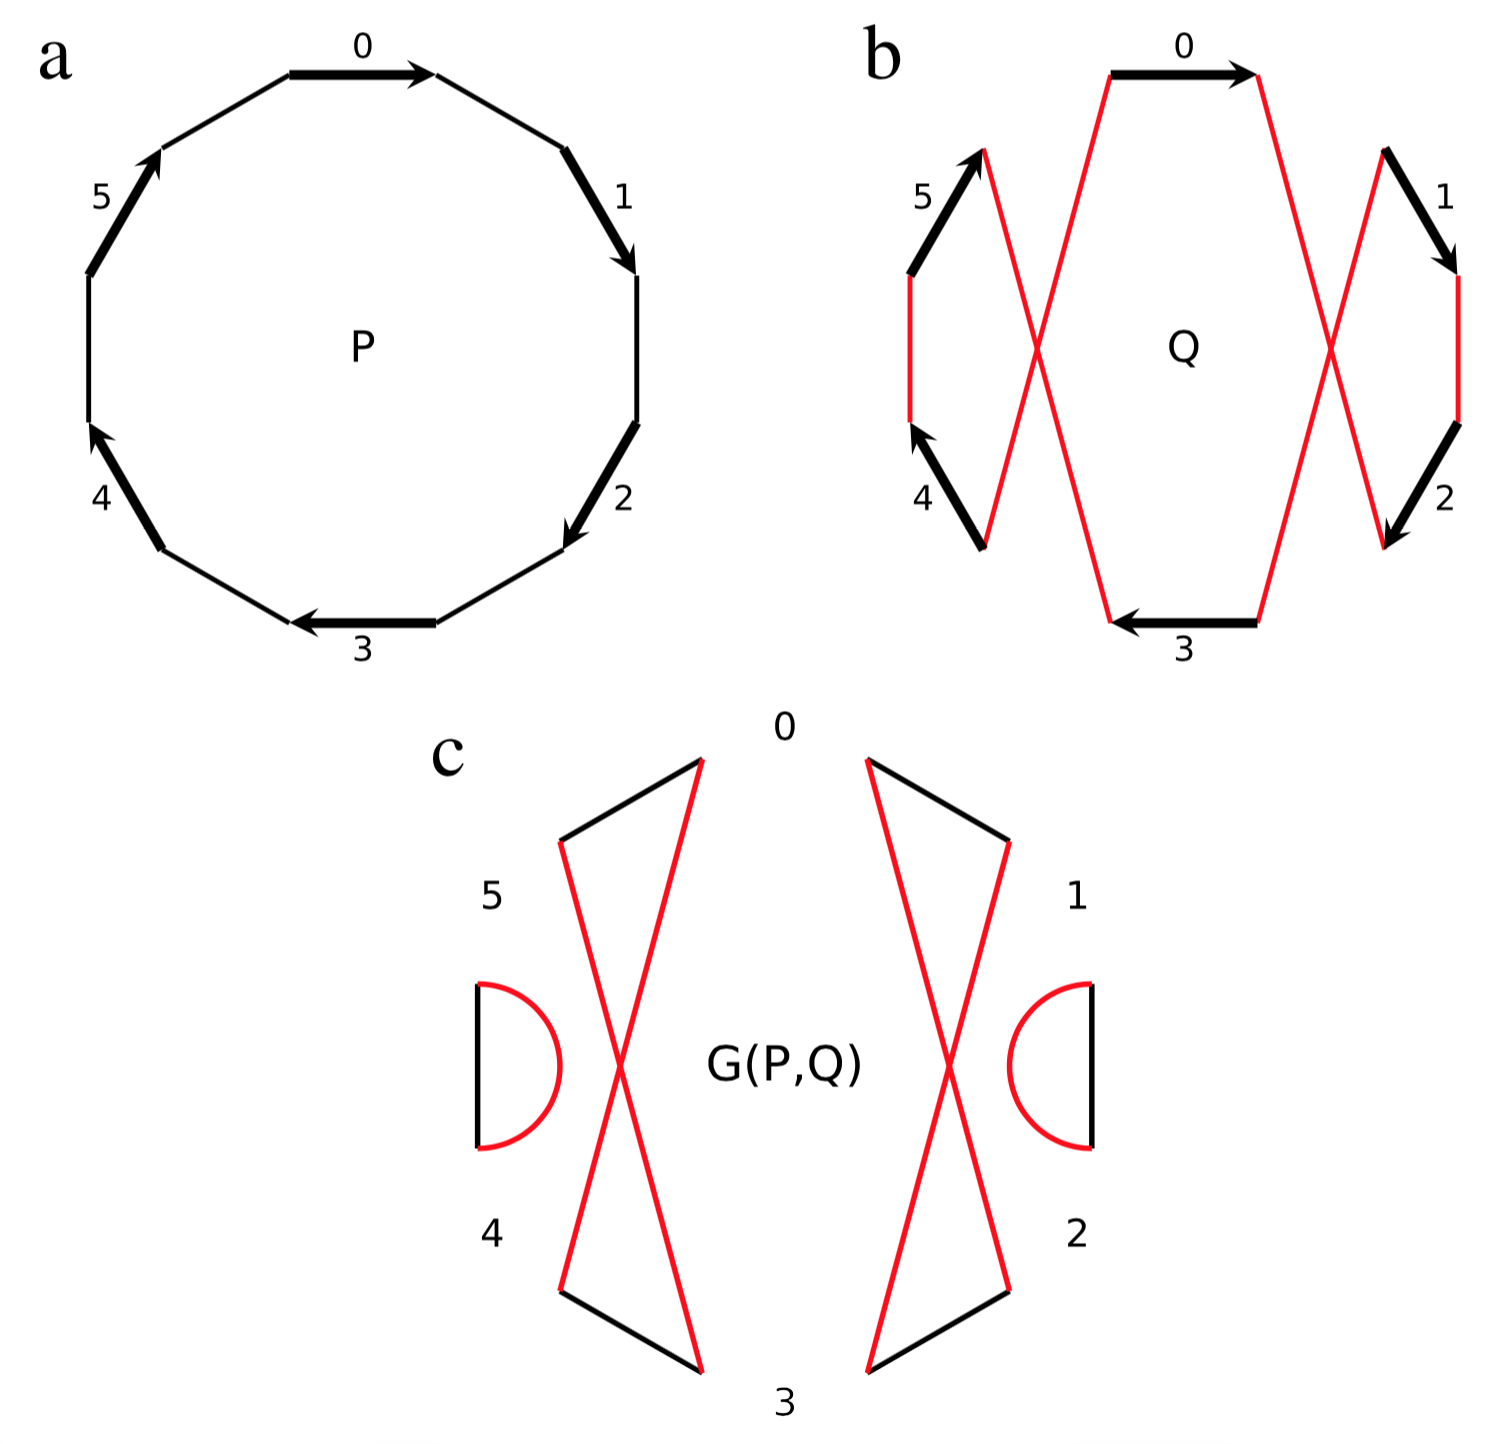
\includegraphics[width=4in]{img/genome_graph.png}
    \caption{
        \textbf{a} Геномный граф однохромосомного генома $P = (0, 1, 2, 3, 4, 5)$ с рёбрами смежности, окрашенными в черный цвет;
        \textbf{b} Геномный граф однохромосомного генома $Q = (0, -2, -1, 3, -5, -4)$ с рёбрами смежности, окрашенными в красный цвет;
        \textbf{c} Граф точек разрыва $G (P, Q)$ геномов $P$ и $Q$ представляет собой набор черно-красных циклов
        }
    \label{al-fig-1}
\end{figure}

Пусть $P$ и $Q$ --- геномы, содержащие один и тот же набор блоков.
Предположим, что в их графах геномов рёбра смежности $P$ окрашены в черный цвет (рис.~\ref{al-fig-1}a), а рёбра смежности $Q$ окрашены в красный цвет (рис.~\ref{al-fig-1}b).
Граф точек разрыва $G (P, Q)$ является суперпозицией графов генома $P$ и $Q$ с удаленными блоковыми рёбрами (рис.~\ref{al-fig-1}c).
Черные и красные рёбра смежности в $G (P, Q)$ образуют совокупность чередующихся черно-красных циклов.

Будем говорить, что черно-красный цикл является $l$-циклом, если он содержит $l$ черных ребер (и $l$ красных), а $c_l (P, Q)$ - число $l$-циклов в $G (P, Q)$. Важно отметить, что мы считаем рёбра только одного цвета, то есть на самом деле мы называем длиной половину числа ребер.
Циклы длины $1$ называют тривиальными, остальные нетривиальными.
Вершины нетривиальных циклов называются точками разрыва (англ. \textit{breakpoints}).

\begin{figure}[h!]
    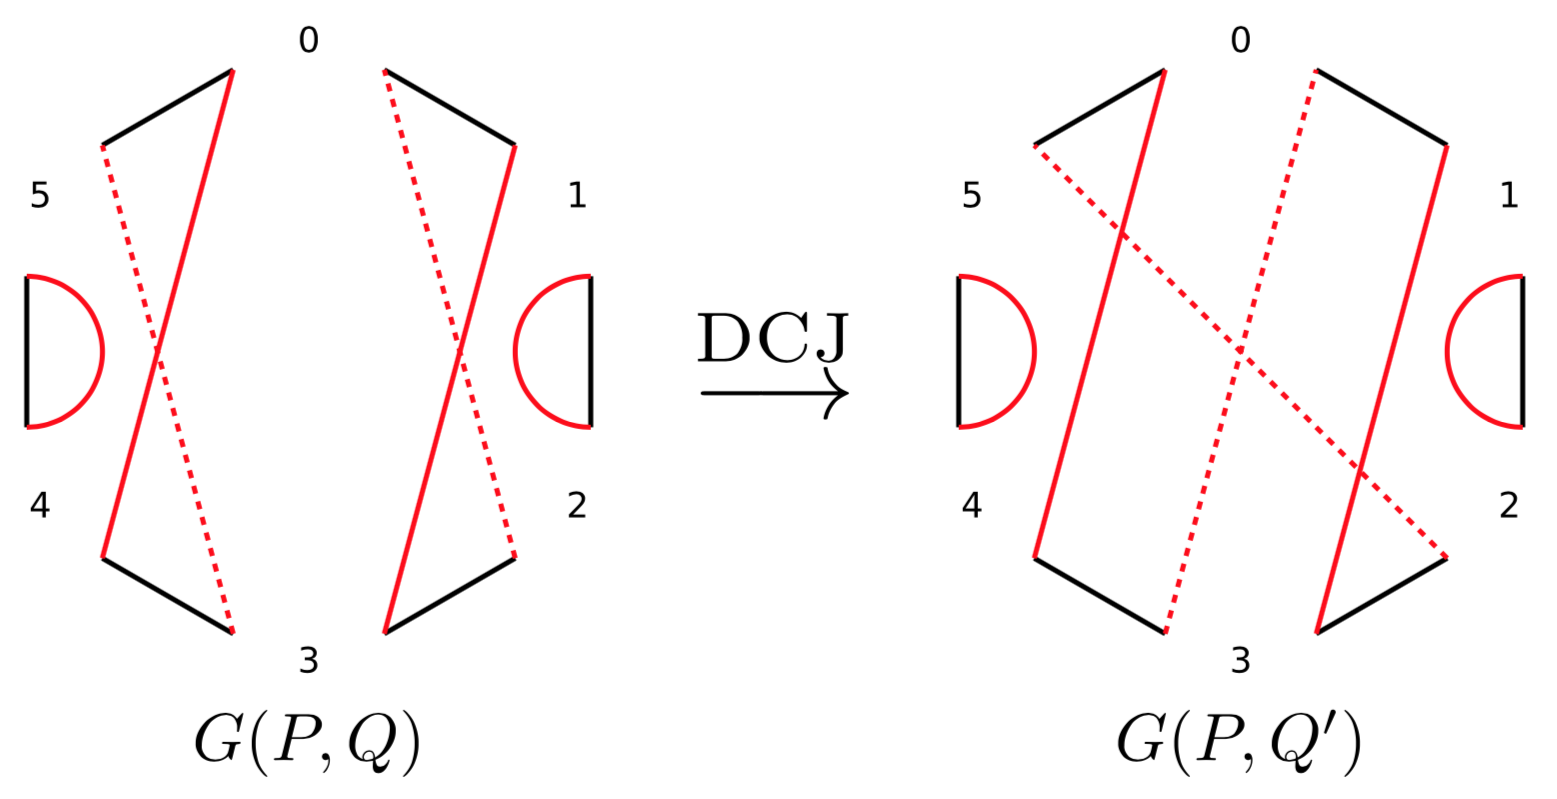
\includegraphics[width=5in]{img/dcj.png}
    \caption{операция ДРС в геноме $Q$ заменяет пару красных ребер в точке разреза $G (P, Q)$ другой парой красных ребер на тех же 4 вершинах}
    \label{al-fig-2}
\end{figure}

Операция ДРС в геноме $Q$ заменяет любую пару красных рёбер смежности $\{x, y\}, \{u, v\}$ другой парой ребер, состоящих из тех же вершин, то есть: $\{x, u\}, \{y, v\}$ либо $\{u, y\} , \{v, x\}$.
Говорится, что такая операция ДРС совершается на ребрах $\{x, y\}, \{u, v\}$ и их конечных точках (англ. \textit{endpoints}) $x, y, u, v$.
Операция ДРС в геноме $Q$, превращающая его в геном $Q'$, соответствует преобразованию графа точек разрава $G (P, Q)$ в граф точек разрыва $G (P, Q')$ (рис.~\ref{al-fig-2}).
Если ребра $\{x, y\}, \{u, v\}$ принадлежат разным циклам, то операция ДРС, осуществляемая на графе точек разрыва, объединяет два цикла в один, а если ребра $\{x, y\}, \{u, v\}$ принадлежат к одному и тому же циклу, то операция ДРС разбивает один цикл на два или сохраняет текущее количество циклов.
Минимальное количество операций ДРС, которое потребуется для преобразования $Q$ в $P$ назовём расстоянием ДРС (обозначается $d(P, Q)$) между геномами $P$ и $Q$.
Также введем ещё две компоненты: $b (P, Q) = \sum_{l \geq 2} l \cdot c_l(P, Q)$ --- половина общей длины всех нетривиальных циклов, $c (P, Q) = \sum_{l \geq 2} c_l(P, Q)$ --- количество циклов длины больше $1$.
Тогда для оценки на $d$ будет достаточно взять их разность: $d (P, Q) = b (P, Q) - c (P, Q)$.

\subsection{Эволюционная модель}
Задача эволюционной модели --- оценка истинного эволюционного расстояния между геномами $P$ и $Q$.
Будем считать, что геномы $P$ и $Q$ имеют один и тот же набор блоков, тогда в качестве процесса эволюции мы можем рассматривать дискретный марковский процесс.
Каждая операция ДРС в таком процессе происходит независимо, то есть у модели нет <<памяти>>, и с их помощью осуществляется последовательное превращение генома $P$ в геном $Q$.
Начальной точкой данного процесса является геном $Z = P$, конечной точкой является геном $Z = Q$.
Подобный процесс будет соответствовать преобразованию графа $G (P, P)$  в граф $G (P, Q)$.
Истинное эволюционное расстояние между $P$ и $Q$ будем оценивать как количество операций ДРС в данном преобразовании (число $k$).

Также важным замечанием является то, что даже при наличии тривиальных циклов в $G (P, Q)$, их количество является неизвестным параметром.
Это связано с тем, что мы не может точно сказать, является ли данный регион <<прочным>> или это <<хрупкий>> регион, который просто не был вовлечен в перестройку.
Для того, чтобы учитывать этот факт будем считать, что геномы $P$ и $Q$  составлены из большого числа $n$ прочных регионов ($n$ неизвестно), сменяющихся хрупкими регионами, причём некоторые регионы могли сохраниться случайно.
Подобные представления геномов $P$ и $Q$ обозначим $P_n$ и $Q_n$.
Далее будем рассматривать преобразование генома $P_n$ в геном $Q_n$ последовательностью операцией ДРС, которые происходят только на хрупких регионах.

Также важно, что, хотя число $n$ прочных областей неизвестно, графы точек разрыва $G (P, Q)$ и $G (P_n, Q_n)$ имеют одну и ту же структуру циклов, за исключением тривиальных циклов.
То есть, мы имеем $c_l (P_n, Q_n) = c_l (P, Q)$ для всех $l \geq 2$, что означает, в частности, $b (P_n, Q_n) = b (P, Q)$ и $c (P_n, Q_n) = c (P, Q)$, а следовательно $d (P_n, Q_n) = d (P, Q)$.
Графы точек разрыва $G (P, Q)$ и $G (P_n, Q_n)$ могут различаться только числом тривиальных циклов, а в нашей модели эта компонента считается неизвестной.

В рамках рассматриваемой эволюционной модели следующие параметры считаются известными, то есть наблюдаемыми:
\begin{enumerate}
    \item $c_l = c_l (P, Q)$ для $l \geq 2$ --- число циклов длины $l$ в $G (P, Q)$;
    \item $b = b (P, Q) = \sum_{l \geq 2} l \cdot c_l$ --- половина от общей длины всех циклов где $l \geq 2$ в $G (P, Q)$;
    \item $d = d (P, Q) = b - \sum_{l \geq 2} c_l(P, Q)$, --- минимальное необходимое количество операций ДРС (для преобразования $P$ в $Q$).
\end{enumerate}

Неизвестными, то есть ненаблюдаемыми, являются следующие параметры:
\begin{enumerate}
    \item $c_1 = c_1 (P_n , Q_n)$ --- число тривиальных циклов в $G(P_n , Q_n)$;
    \item $n$ --- половина общей длины всех циклов в $G(P_n , Q_n)$ или число хрупких регионов в геномах $P$ и $Q$;
    \item $k = k(P, Q)$ --- чило ДРС операций в Марковском процессе или истинное эволюционное расстояние между $P$ и $Q$.
\end{enumerate}

В качестве замечания необходимо отметить, что данная модель легко применяется к линейным геномам простым добавлением ребра между последним и первым блоками.

\subsection{Теоретический анализ и оценка расстояния}
В рамках данной модели основной задачей является оценка неизвестных параметров через известные.
Для всех необходимых компонент аналитически выведем необходимые формулы.

Количество циклов заданной длины можно посчитать по формуле:
$$c'_{n,k,m}=
\frac{\binom{k}{m-1}\binom{n-m}{2}^{k-m+1}m^{m-2}m!}
{\binom{n}{2}^k},$$
где $n$ --- число вершин, $k$ --- число шагов, $m$ --- длина цикла

Переходя к пределу, получим:
$$\frac{c_l} n = \frac {c'_{n,k,m}} n \xrightarrow[n \to \infty]{[k=\frac{n \gamma}{2}]} \frac{e^{-\gamma l} \gamma^{l-1} l^{l-2}} {l!},$$
где $\gamma = \frac {2k} n$ --- число произошедших перестроек, нормированное относительно общего числа областей

Далее оцениваются нормированные величины $d$ и $b$:

$$\frac b n = 1 - e ^ {- \gamma} + o(1)
\qquad
\frac d n = 1 - \sum_{l=1}^{\infty} \frac {p_l} l + o(1),$$
$$p_l = e^{-\gamma l} \frac {(\gamma l)^{l-1}}{l!}$$

После этого мы можем оценить величину $\frac d b$ отдельно от $n$:
$$\frac d b \approx  \frac {1 - \sum_{l=1}^{\infty} e^{-\gamma l} \frac {(\gamma l)^{l-1}}{l \cdot l!}}{1 - e ^ {- \gamma}} \, .$$

Но величины $d$ и $b$ известны в рамках данной модели, и мы знаем формулу зависимости $\gamma$ от этих величин.
А также известно, как величина $\frac b n$ зависит от $\gamma$.
Зная эти зависимости, получаем формулу для неизвестных нам $n$ и $k$:
$$n_e = \frac b {1 - e^{-\gamma_e}}
\qquad
k_e = \frac {\gamma_e \cdot n_e} {2},$$
\centerline{где $n_e$ --- оценка на количество хрупких регионов,}
\centerline{$k_e$ --- оценка на истинное эволюционное расстояние}

\begin{figure}[h!]
    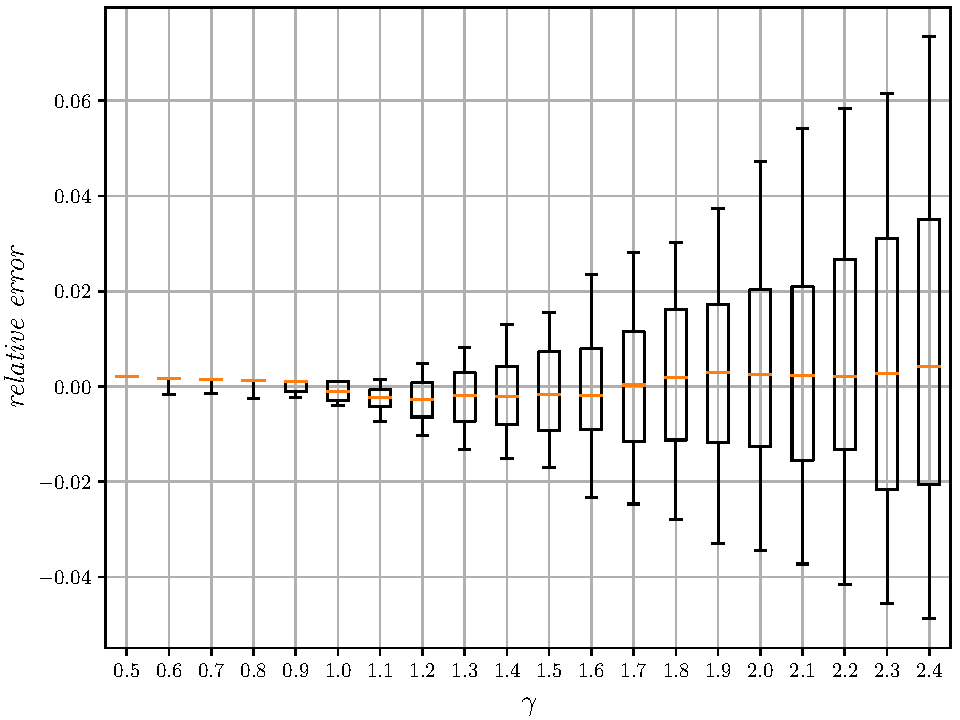
\includegraphics[width=.8\linewidth]{img/classic_est_error.pdf}
    \caption{Зависимость распределения относительной ошибки $\frac {k_e - k} k$ от $\gamma$ }
    \label{classic-est-error}
\end{figure}
Для оценки качества работы данного метода проведём 200 независимых экспериментов с моделируемым Марковским процессом построим график вида <<ящик с усами>> (рис.~\ref{classic-est-error}).

На данном графике и во всех подобных графиках далее <<ящикам>> соответствует $50 \, \%$ результатов, а усам $90 \, \%$.
Как мы видим, данный метод в $90 \, \%$ случаев ошибается не более, чем на $7 \, \%$, что является отличным показателем.
Но, к сожалению, данная модель имеет и недостатки, критика была высказана в \cite{fr-4}.

Дело в том, что выбор рёбер в Марковском процессе происходит равновероятно, в то время как в реальной жизни некоторые регионы имеют больший шанс быть вовлеченными в перестройку, а некоторые меньшую.
Данное замечание послужило мотивацией для создания модели, представленной  в данной работе.

\section{Описание модели Дирихле}

\subsection{Снабжения графа точек разрыва весами}
Аналогично ПХР-модели модель Дирихле использует граф точек разрыва для представления геномов.
В данной модели мы будем считать, что у каждого хрупкого региона есть некоторая вероятность быть вовлеченным в перестройку.

\begin{figure}[h!]
    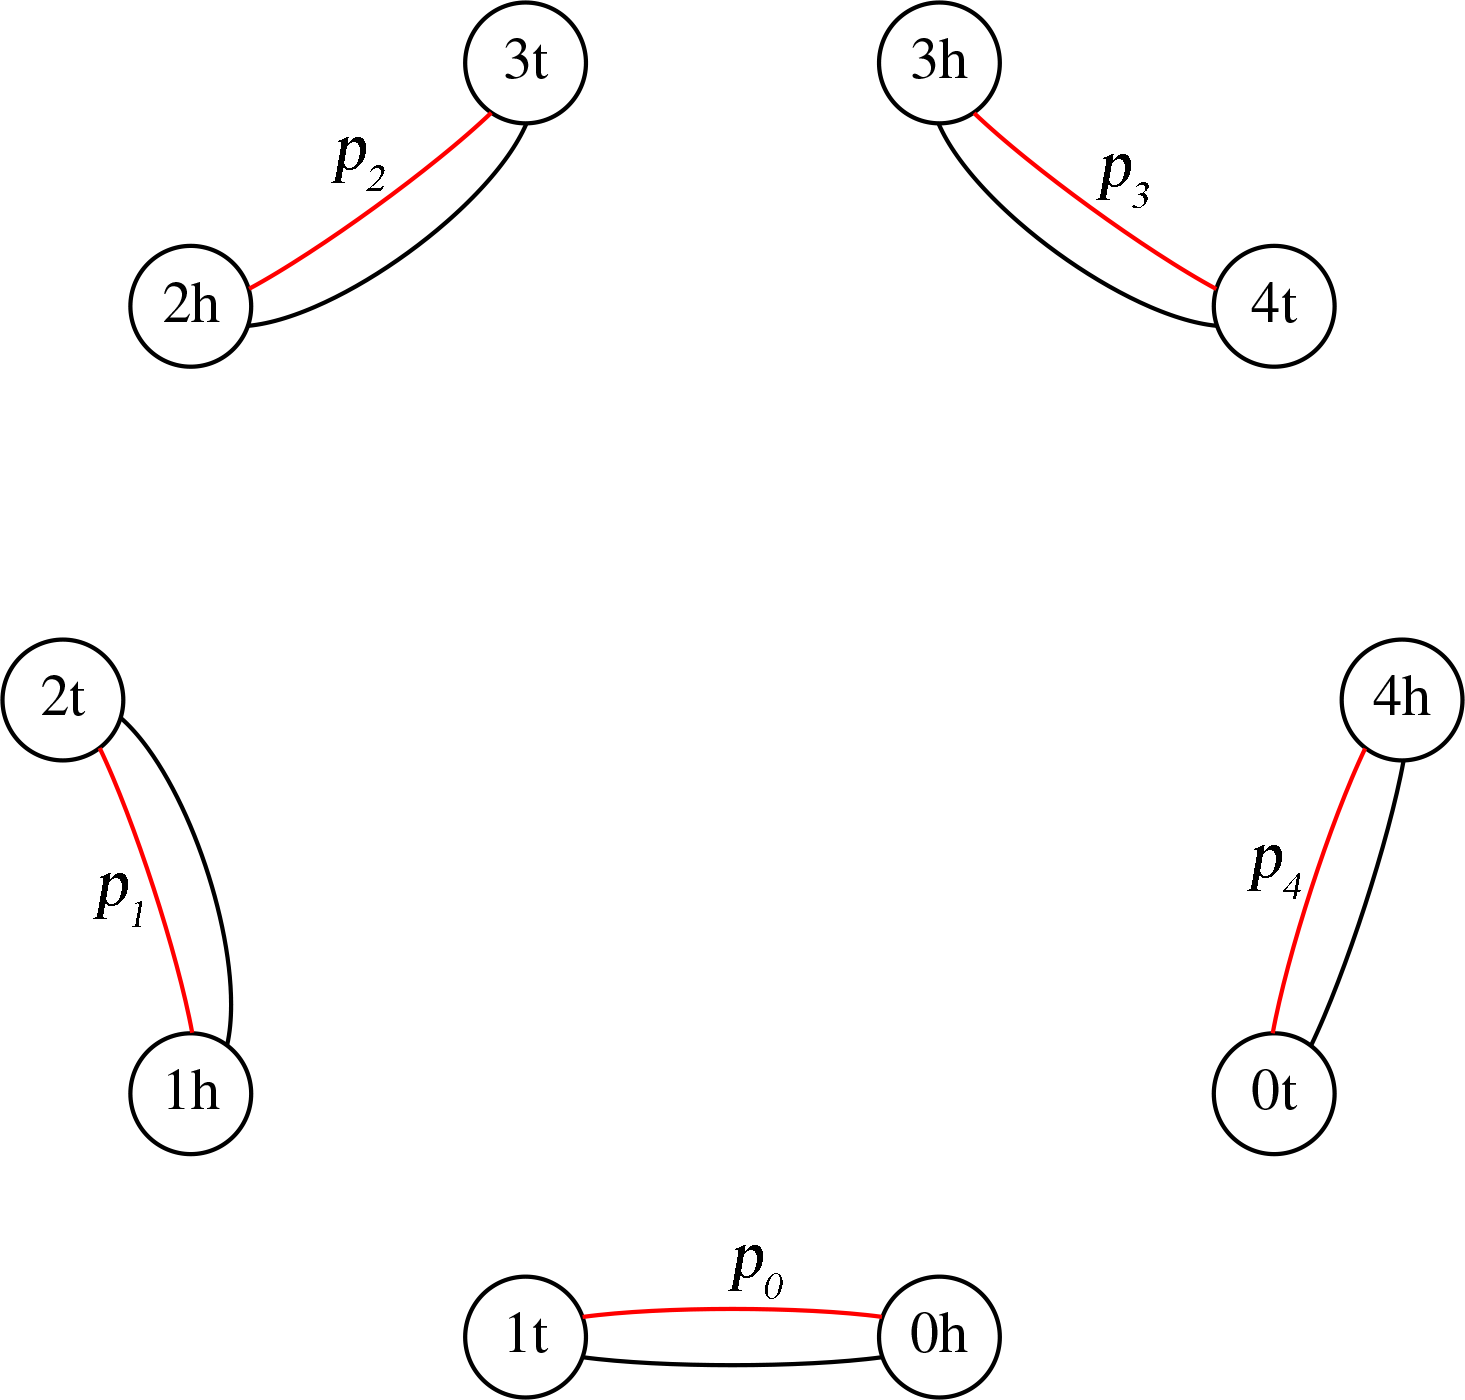
\includegraphics[width=4in]{img/bpg0-eps-converted-to.png}
    \caption{Граф точек разрыва с весами}
\end{figure}

Пусть $n$ --- это размер геномов $P$ и $Q$.
Каждое красное ребро в графе снабдим соответствующим числом $p_i$ --- его вероятностью быть вовлеченным в перестройку.
$\sum_{i=0}^{n-1} {p_i} = 1$ по определению.

\subsection{Модификация операции двойной-разрез-и-склеивание}
Операция ДРС также производится на красных ребрах.
Но теперь помимо рёбер смежности она принимает и вероятности, подписанные на этих ребрах.

Пусть операция ДРС производится на рёбрах с номерами $i$ и $j$ и соответствующие рёбра смежности --- это $\{x, y\}, \{u, v\}$, а вероятности --- $p_i$ и $p_j$.
Эта операция аналогично заменяет данные рёбра другой парой рёбер, образующих паросочетания на тех же вершинах, что и исходные, то есть $\{x, u\}, \{y, v\}$ либо $\{u, y\} , \{v, x\}$.
Также перераспределяются и веса.
Новые веса $p_i'$ и $p_j'$ будут равны $r_1 \cdot p_i + r_2 \cdot p_j$ и $(1 - r_1) \cdot p_i + (1 - r_2) \cdot p_j$ соответственно, где $r_1$ и $r_2$ --- случайные числа из отрезка $(0, 1)$.

\begin{figure}[h!]
    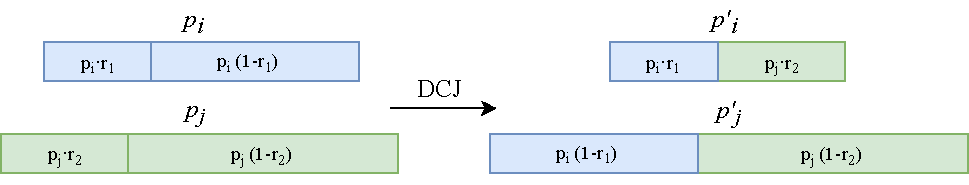
\includegraphics[width=\linewidth]{img/weights-redistribution.pdf}
    \caption{Пример перераспределения весов}
    \label{weights-redistribution}
\end{figure}

Указанное перераспределение весов предложено в статье \cite{fr-4}, и соответствующие веса и правила перераспределения весов обусловлены биологически.
В реальной жизни вероятность поломки какого-либо региона зависит от множества факторов.
Геном имеет достаточно сложную трёхмерную структуру \cite{3d} и вероятность поломки региона тесно связана с физическим устройством генома.
В данной работе мы придерживаемся мнения о том, что хрупкие регионы являются участками открытого хроматина.
В предположении, что хрупкие регионы являются участками открытого хроматина, хрупкий регион может сломаться в любом своём месте. Считается, что вероятность быть вовлеченным в перестройку пропорциональна длине этого региона.

Каждый регион, вовлеченный в перестройку, равновероятно ломается в случайном месте своей длины, что соответствует числам $r_1$ и $r_2$.
И далее веса перераспределяются в соответствии с местами этих поломок, сохраняя общую сумму вероятностей (для примера см. Рис.~\ref{weights-redistribution}).

\subsection{Эволюционная модель и равновесное распределение}
Как и в ПХР-модели, рассмотренной ранее, для оценки истинного эволюционного расстояния между геномами $P$ и $Q$, которые имеют один и тот же набор блоков, будем рассматривать процесс эволюции как дискретный Марковский процесс, который начинается с генома $P$ и заканчивается геномом $Q$.
Подобное преобразование, как и ранее, осуществляется с помощью последовательности операций ДРС.

Отличие заключается в том, что на каждом шаге Марковского процесса выбор ребра происходит не равновероятно, а соответствует вероятностям, написанным на соответствующих рёбрах.
То есть вероятность того, что $2$ ребра с номерами $i$ и $j$ будут вовлечены в перестройку, будет равна $p_i \cdot p_j$ (выбор происходит независимо).

Полученный марковский процесс является:
\begin{enumerate}
    \item Реверсивным, то есть время возвращения в некоторое состояние имеет конечное математическое ожидание;
    \item Непериодичным, так как существует ненулевая вероятность остаться в текущем состоянии;
    \item Неразложимым, то есть любое состояние процесса может быть достигнуто из любого другого состояния за конечное число шагов. Это свойство может быть проверено простым упорядочиванием состояний и математической индукцией. \\
\end{enumerate}
Следовательно, этот марковский процесс сходится \cite{teor-ver}.
Как показано в \cite{fr-4}, стационарное распределение этого процесса -- это равномерное распределение на всех векторах $p = \{p_i\}$, сумма которых равна $1$.
Это распределение является плоским распределением Дирихле.

Для того, чтобы получить данное распределение, достаточно выбрать отдельные вероятности как распределенные по экспоненциальному закону и нормализовать \cite{generation}:
$$\text{Пусть} \, i \in \{1, 2, \ldots, n\}, \qquad \alpha_i = Exp(1), \qquad M = \sum_{i=0}^n \alpha_i,$$
$$\text{тогда} \,\, (p_1, p_2, \ldots, p_n) 
= \left(\frac {\alpha_1} M, \frac {\alpha_2} M, \ldots, \frac {\alpha_n} M\right) 
= Dir(1, 1, \ldots, 1).$$

\chapterconclusion
В главе 1 были рассмотрены известные на данный момент методы для оценки эволюционного расстояния: оценка через минимальное расстояние, модель поломки случайных регионов, модель поломки хрупких регионов. Несмотря на то, что в рамках рассмотренных моделей можно получать достаточно точные результаты относительно истинного эволюционного расстояния, все они не учитывают некоторых биологических особенностей генома, например, факт того, что разные хрупкие регионы могут иметь разную вероятность быть вовлеченными в перестройку.

Была описана модель устройства генома, более точно учитывающая структуру ДНК (модель Дирихле). В дальнейшем будет проведён анализ именно этой модели.